En las últimas décadas se ha observado un movimiento global hacia sistemas de cultivo automatizados capaces de incrementar la calidad y efectividad de producción de cultivos. Factores como la urbanización, el crecimiento poblacional y el cambio climático han promovido el desarrollo de nuevas tecnologías de cultivo para reducir su consumo de agua y espacio requerido.

Uno de los sistemas más prometedores es el cultivo hidropónico. Estos cultivos requieren de entornos controlados y soluciones de fertilizantes en agua para lograr el crecimiento de hortalizas sin la necesidad de sustratos convencionales. La reducción en espacio y agua requerida para estos cultivos, así como su requisito de un control ambiental específico, han facilitado su integración con diferentes tecnologías para su automatización. Ciertas plataformas automatizadas para cultivos hidropónicos han sido desarrolladas e implementadas exitosamente. Sin embargo, en Guatemala, este campo de estudio aún se encuentra en desarrollo.

\subsection*{La hidroponía en Guatemala}
Actualmente, el mercado de cultivos e infraestructuras hidropónicas en Guatemala sigue en sus etapas iniciales. Mientras que existen cultivos hidropónicos en diferentes sectores agro-industriales, esta metodología no ha sido ampliamente implementada.

En la Universidad del Valle de Guatemala, se realizó un estudio que buscó determinar las oportunidades de crecimiento y la demanda existente en el mercado para cultivos producidos en una granja urbana empleando metodologías hidropónicas. \cite{gonzalez_natareno2021_tesis} Dicho estudio buscó determinar la viabilidad económica de un sistema de cultivo hidropónico en Quetzaltenango mediante estudios de mercado y el diseño de un sistema para el cultivo de hortalizas de hoja. Se analizaron factores como la ubicación, espacio requerido, variedades de sistemas hidropónicos existentes, la segmentación del mercado, entre otros. Adicionalmente, se realizó un diseño preliminar de un sistema hidropónico utilizando la metodología NFT (Nutrient Film Technique) implementando una configuración de invernadero con túneles. La metodología NFT mantiene un flujo constante de agua sobre las raíces de manera que estas estén levemente cubiertas. Esta metodología mejora la oxigenación de las raíces y permite que estas absorban la cantidad necesaria de nutrientes. 

Al analizar los resultados de los estudios técnicos y financieros realizados, se determinó que existe un mercado disponible en el área de Quetzaltenango para la venta de cultivos hidropónicos. Adicionalmente, los resultados presentaron una alta rentabilidad para el proyecto con una tasa interna de retorno (TIR) de 128.07\% lo cual indica la factibilidad positiva de los sistemas hidropónicos en Guatemala. Cabe mencionar que este estudio consideró un sistema hidropónico manual en donde las variables estarían siendo controladas por un equipo de trabajo capacitado.

\begin{figure}[H]
	\centering
	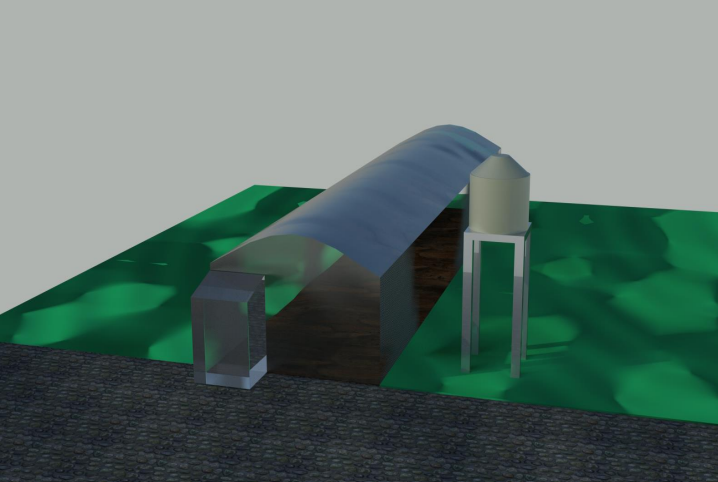
\includegraphics[scale= 0.5]{Figura1_modelo3D_invernadero_gonzalez.png}
	\caption{Modelo 3D de invernadero propuesto en estudio de factibilidad de cultivos hidropónicos.}
	\label{fig:mesh1}
\end{figure}

\subsection*{Tendencias actuales en la producción sostenible de hortalizas}
El concepto de cultivos sin sustrato ha existido en la sociedad desde hace cientos de años. A inicios y mediados del Siglo XVII, diferentes científicos realizaron experimentos para demostrar que las plantas son capaces de crecer suspendidas en soluciones de agua, minerales y otros nutrientes. A mediados del mismo siglo, se encontró la importancia de diferentes sales las cuales ayudan a regular el proceso de crecimiento de las plantas, mejorando su rendimiento y calidad \cite{rajaseger_hydroponics_2023}. 

En la actualidad, diferentes factores como el cambio climático y el crecimiento de la población global han requerido nuevos avances en los sistemas de producción de alimentos. Estos factores han llevado a la implementación de sistemas hidropónicos en diferentes países como una medida para aumentar la producción alimenticia sin sacrificar espacio en sus territorios. Los cultivos hidropónicos presentan una gran ventaja al ser un método de cultivo altamente controlable, lo cual aumenta la productividad de un terreno. Adicionalmente, diferentes configuraciones permiten la producción de un mayor volumen de hortalizas en espacios reducidos. Junto a esto, estas metodologías reducen el impacto ambiental del cultivo de alimentos al eliminar la necesidad de alterar ecosistemas para la instalación de plantaciones masivas, y reducir el consumo de agua.

\begin{figure}[H]
	\centering
	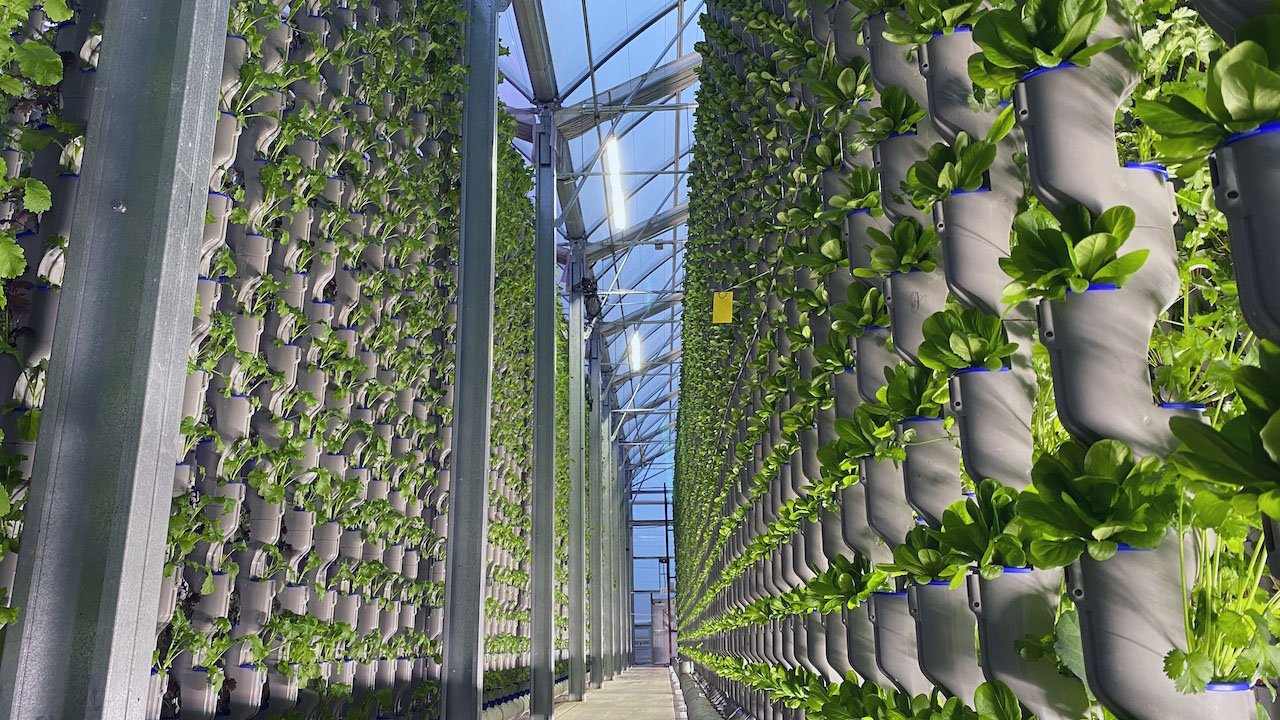
\includegraphics[scale= 0.25]{Figura3_vertical-greenhouse_edengreen.jpg}
	\caption{Granja hidropónica vertical de \textit{Eden Green}. \cite{edengreen_10_nodate}}
	\label{fig:mesh2}
\end{figure}

En el estudio de Rajaseger y colaboradores \cite{rajaseger_hydroponics_2023}, se detallaron las tendencias recientes más relevantes alrededor de la integración de cultivos hidropónicos con tecnologías inteligentes. Se destaca cómo la hidroponía es capaz de reducir el consumo de agua, minimizar el impacto ambiental de la agricultura y mejorar la calidad de los productos mientras ahorra energía y reduce tanto el espacio como la mano de obra requeridos para su producción. Adicionalmente, presenta esta tecnología como uno de los mejores candidatos para lidiar con los retos del Siglo XXI al permitir su implementación en entornos urbanos, en especial, al considerar la tendencia actual de urbanización. Se presentaron los diferentes métodos de cultivo hidropónico que se han desarrollado en los últimos años así como un resumen de los desarrollos tecnológicos en la integración de agricultura inteligente e hidroponía. Se detalló cómo varios estudios, buscando determinar la factibilidad de la hidroponía para producción sostenible, han incorporado diferentes sensores para medir características como niveles de oxígeno o pH en el agua. Estos componentes, junto con sistemas de control, permiten monitorear una gran cantidad de variables internas y externas, y controlarlas para obtener mejores resultados. Se realizó una recopilación respecto a la importancia de diferentes medios de crecimiento sólidos y nutrientes en el desarrollo de las plantas en entornos hidropónicos. Finalmente, los autores hacen énfasis en el valor de esta nueva tecnología para la producción local de alimentos en áreas urbanas. \say{Esta estrategia novedosa podrá llegar a alterar de manera significativa el sector agricultural al incentivar la producción regional de alimentos, mejorando la seguridad alimenticia y añadiendo a metodologías de cultivo más resilientes.} (\textit{Rajaseger et al.}, 2023, p. 926)

\subsection*{Uso de \textit{Fuzzy Logic} para el control de sistemas hidropónicos}
Los sistemas hidropónicos manejan una gran cantidad de variables las cuales deben ser controladas de tal manera que se mantengan en rangos preestablecidos. Debido a la gran variedad de plantas que se pueden cultivar en un sistema hidropónico se requieren controladores con rangos que se puedan adaptar, según el cultivo seleccionado. Los controladores que emplean \textit{fuzzy logic} son capaces de alterar sus rangos de control de manera dinámica y con facilidad. Dichos controladores permiten definir rangos de entrada los cuales pueden ser mapeados a rangos de salida. Al momento de evaluar el estado del sistema, se utilizan funciones específicas para realizar una linealización aproximada de las variables medidas. En base a estas linealizaciones se determina la compensación que debe realizar el controlador para mantener los niveles deseados. Esto permite una fácil integración con sistemas IoT (\textit{Internet of Things}) puesto que los rangos pueden ser variados por el usuario según los requisitos del sistema.

\begin{figure}[H]
	\centering
	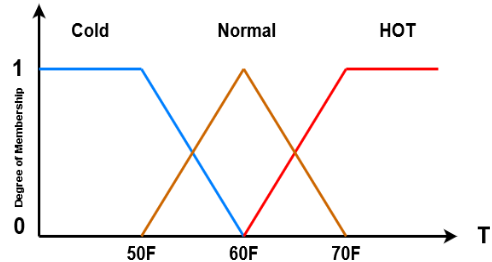
\includegraphics[scale= 0.75]{Figura4_funcion-membresia-fuzzy-logic.png}
	\caption{Función de membresía de entradas de temperatura para \textit{fuzzy logic}. \cite{thazin_iot_2019}}
	\label{fig:mesh3}
\end{figure}

\indent En el estudio de Thazin y colaboradores \cite{thazin_iot_2019}, se implementó un controlador utilizando \textit{fuzzy logic} para regular la temperatura y humedad de un sistema hidropónico mediante cambios al flujo de aire en el entorno. Se realizaron cálculos de los ventiladores DC requeridos para alterar los parámetros deseados, los cuales se instalaron en posiciones estratégicas dentro del entorno de crecimiento diseñado para mejorar el flujo de aire. Se utilizó un Arduino Nano junto con un sensor DHT22 para realizar las mediciones de temperatura y controlar la velocidad de los ventiladores. Adicionalmente, se incluyó una pantalla LCD como display para las mediciones de temperatura y velocidad de los ventiladores. Con el controlador propuesto se logró un control adecuado de la velocidad de los ventiladores en función del rango de temperatura ambiente en el área de crecimiento. Se demostró que el sistema fue capaz de variar la velocidad angular de los ventiladores utilizados según la temperatura mediante la realización de 10 pruebas a temperaturas entre los 45 y 87 °F. Adicionalmente, se logró subir los resultados a la plataforma \textit{Thing Speak} para monitorear valores de temperatura, humedad e intensidad de luz. Dicha plataforma cuenta con un servidor al cual se pueden subir datos mediante protocolos WiFi para que estos sean desplegados en gráficas en función del tiempo transcurrido.

\subsection*{Monitoreo y control de cultivos hidropónicos utilizando tecnología IoT}
El monitoreo de las variables presentes en sistemas hidropónicos es esencial para asegurar un crecimiento óptimo de las hortalizas. Sin embargo, este proceso puede llegar a consumir mucho tiempo en el caso de sistemas a mayores escalas y puede ser ineficiente en lugares remotos. Por esta razón, el estudio de Tatas y colaboradores \cite{tatas_reliable_2022} buscó desarrollar un sistema de monitoreo y control automático de parámetros de calidad de agua y condiciones ambientales para un cultivo hidropónico en invernadero. Adicionalmente, se definió como objetivo lograr que este aprovechara tecnologías IoT para la transferencia y el análisis de datos. Se definieron requerimientos para el sistema como parámetros a monitorear, períodos de muestreo y acciones o alarmas según los diferentes eventos. Luego de la selección de los sensores que se utilizarían, en función de los parámetros que se irán a monitorear y considerando una baja frecuencia de re-calibración, se implementó una red de nodos sensoriales. Se configuró la conexión entre nodos de tal manera que todos transmitieran su señal a un solo dispositivo. Esto permitió una comunicación eficiente entre el controlador principal y los monitores de estado (sensores) sin el uso de conexiones físicas. Se realizaron mediciones de consumo eléctrico mediante las cuales se determinó un consumo máximo para la unidad principal de 11.5W bajo condiciones de alta demanda, principalmente debido a la transmisión de datos por el módulo GSM/GPRS. Luego de esto, se desarrolló un controlador implementando \textit{Fuzzy Logic} con tal de activar las bombas de circulación en los momentos adecuados. Se evaluaron los resultados tanto en pruebas de laboratorio como en el campo al instalar el sistema en un invernadero para simular condiciones reales. Se desplegaron los datos recolectados en la plataforma Ubidots y se realizaron pruebas de factibilidad del sistema. Se determinó que, tanto el sistema como los sensores, cuentan con una probabilidad de falla relativamente baja lo cual hace del sistema altamente confiable. 

\begin{figure}[H]
	\centering
	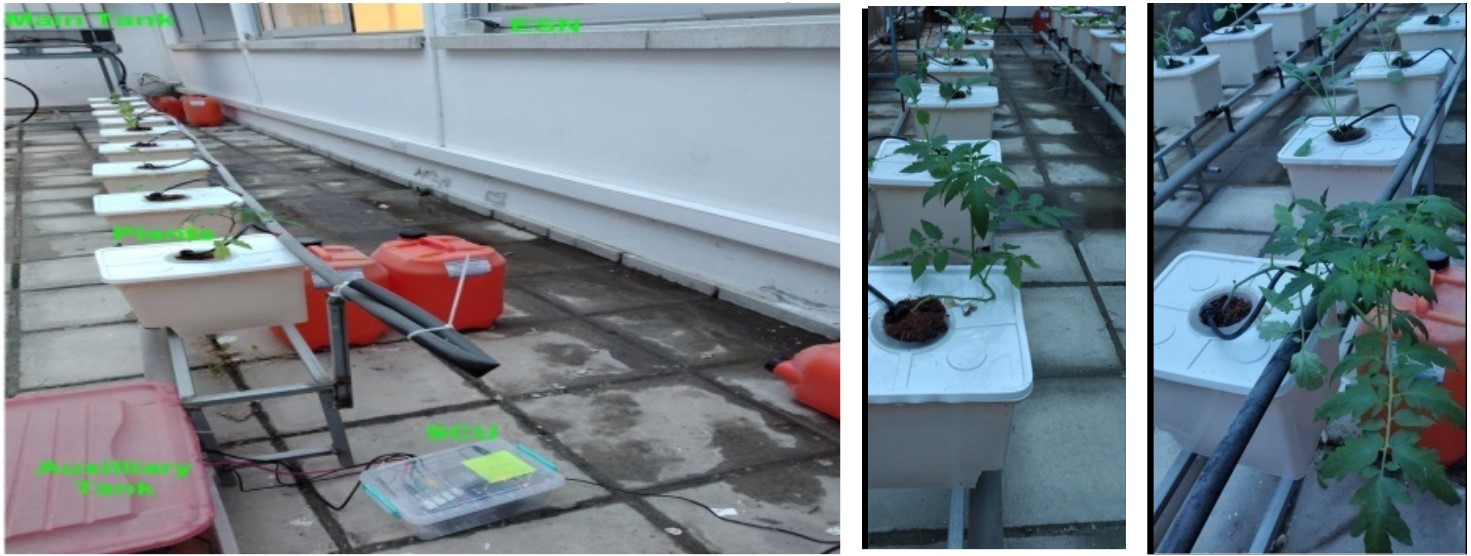
\includegraphics[scale= 0.35]{Figura2_sistema_hidroponico_en-lab_tatas.jpg}
	\caption{Sistema hidropónico implementado en condiciones de laboratorio.}
	\label{fig:mesh4}
\end{figure}

\subsection*{La digitalización de la agricultura}
En los últimos 20 años se ha observado una tendencia hacia la automatización de la agricultura y el concepto de las granjas inteligentes \textit{Smart Farms (SF)}. Mientras que esta tendencia es bastante reciente, siendo popularizada alrededor de los años 90 del siglo pasado, se han empezado a desarrollar tecnologías que están facilitando su implementación. 
\\ En el estudio de Bacco y colaboradores \cite{bacco_digitisation_2019}, realizado en la Unión Europea en el año 2019, se analizaron las tendencias tecnológicas junto con los retos a los que se enfrenta la agricultura moderna en el contexto de la globalización y el calentamiento global. Adicionalmente, se analizaron los retos a los que se enfrentan las tecnologías de granjas inteligentes en desarrollo. Se destacaron factores como costos elevados de adopción de las tecnologías, así como falta de conectividad en áreas rurales. Así mismo, se analizaron factores técnicos y socio-económicos que están afectando la adaptación de los sistemas de agricultura tradicional a metodologías automatizadas. Un aspecto clave que se mencionó fue la tendencia de estas tecnologías hacia un sistema excesivamente industrializado, el cual tiende a desanimar a los agricultores. Sin embargo, como se menciona en el artículo, \say{-el objetivo de las granjas inteligentes (SF) no debería restringirse a la industrialización de la agricultura, sino en mejorar el proceso entero para que este sea más eficiente, sostenible y de mejor calidad, mientras que se respetan las necesidades de los agricultores.} (Bacco \textit{et al.}, 2019, p. 1), estos sistemas pueden ser diseñados de tal manera que sean más compatibles con las necesidades puntuales de los agricultores. %\vspace{10pt}
%\textit{-the aim of SF should not be just in industrializing agriculture, but in making the whole process more efficient, sustainable, and of high quality, while respecting farmers’ needs.}

\indent La hidroponía ha presentado grandes avances a lo largo de los últimos años, desde sus inicios teóricos en el Siglo XVII hasta el crecimiento en popularidad en años recientes, esta tecnología se encuentra posicionada para ser revolucionaria en la agricultura moderna. Actualmente, existen diversas empresas las cuales están demostrando los beneficios de esta tecnología junto con su viabilidad. Adicionalmente, varios estudios han comprobado su factibilidad y el potencial presente en la integración con sistemas inteligentes. El campo de la automatización agrícola se ha encontrado en crecimiento a lo largo de los últimos 20 años, y los cultivos hidropónicos presentan una plataforma idónea para su implementación en los años por venir. Tanto el calentamiento global como la urbanización han sido reconocidos como retos que pueden llegar a aumentar la falta de seguridad alimenticia en esta y futuras generaciones. Por esta razón, es de gran importancia mejorar los protocolos de automatización y sistemas de control para facilitar la adopción de los cultivos hidropónicos tanto en Guatemala como en Latinoamérica.
